\documentclass[12pt]{book}
\usepackage[margin=.85in]{geometry} % for MARGIN
\usepackage[many]{tcolorbox}    	% for COLORED BOXES (tikz and xcolor included)

\usepackage{multirow}
\usepackage{tabularx}
\usepackage{multicol}   
\usepackage{enumerate}
\usepackage[shortlabels]{enumitem}
\usepackage{varwidth}
\usepackage{tasks}
\usepackage[export]{adjustbox}
\usepackage{array} % For m{} column type

\usepackage{titleps}
\usepackage{setspace}               % for LINE SPACING
\usepackage[⟨options⟩]{fancyhdr}
\usepackage{enumitem}
\setlist{nosep}
\usepackage{tikz}
\usepackage{pgfplots}
\pgfplotsset{compat=1.5.1}
\usetikzlibrary{datavisualization}
\usetikzlibrary{datavisualization.formats.functions}

\newcommand{\D}{\displaystyle}
\newcommand\Mydiv[2]{%
$\strut#1$\kern.25em\smash{\raise.3ex\hbox{$\big)$}}\mkern-8mu
        \overline{\enspace\strut#2}}


\setlength\parindent{0pt}   % killing indentation for all the text
\setstretch{1.3}            % setting line spacing to 1.3
\setlength\columnsep{0.25in} % setting length of column separator
\pagestyle{fancy}           % setting pagestyle to be headings

\usepackage[]{titlesec}

\fancyhead[L]{Math V04 - College Algebra}
\fancyhead[R]{Christina Papazacharioudakis}

\tcbset{
    sharp corners,
    colback = white,
    before skip = 0.2cm,    % add extra space before the box
    after skip = 0.5cm      % add extra space after the box
}                           % setting global options for tcolorbox

    \newtcolorbox{boxR}{
    fontupper = \color{black}, % font color
    boxrule = 1.5pt,
    colframe = black,
    rounded corners,
    arc = 5pt   % corners roundness
}



\begin{document}


{\Large \textbf{5.6 Rational Functions}}


In this section, we will study the graphs of rational functions. So what is a ratioinal function?

\begin{boxR}
    A \textbf{rational function} is a function that can be written as the quotient of two polynomial functions, $P(x)$ and $Q(x)$. 

    $$f(x) = \frac{P(x)}{Q(x)}$$

    where $Q(x) \neq 0$. The \textbf{domain} of a rational function is the set of all real numbers except the $x$-values that make the denominator zero. 
\end{boxR}


\textbf{{\large Finding the Domain of Rational Functions}}
Finding the domain of a rational function means excluding values that make the denominator zero. For example, the domain of the rational function $$ f(x) = \frac{x^2+7x+9}{x(x-2)(x+5)}$$
\vspace{2mm}

is the set of all real numbers except for: \underline{\hspace{25mm}}
\vspace{2mm}

\underline{\textbf{Example 1 - Find the Domain of the Given Functions}}

Find the domain of each rational function and state the answer in interval notation. 
\vspace{2mm}
    \begin{enumerate}[(a)]
        \item $\D f(x)= \frac{x^2-9}{x-3}$
            \vspace{25mm}
        \item $\D f(x)= \frac{x}{x^2-9}$
            \vspace{25mm}
        \item $\D f(x)= \frac{x+3}{x^2+9}$
            \vspace{25mm}
    \end{enumerate}


\newpage
The most basic rational function is the toolkit function $\D f(x)= \frac{1}{x}$. The denominator of the function is zero when $x=0$. The domain of $f$ is the set of all real numbers except for zero. 

Let's look at the behavior of $f$ near the excluded value of $x=0$. 

We start by evaluating $f(x)$ to the left of $0$:
\begin{multicols}{2}
      \renewcommand{\arraystretch}{1.6} % Adjust row height for better vertical alignment
\begin{tabular}{|m{1.5cm}|m{2cm}|} 
         \hline
         $x$ & $f(x)=\frac{1}{x}$  \\ 
           \hline
              $-1$ & $ $ \\
             \hline
             $-0.5$ & $ $ \\
             \hline
            $-0.1$ & $ $ \\
         \hline
            $-0.01$ & $ $ \\
         \hline
           $-0.001$ & $ $ \\
         \hline
        \end{tabular}

        \begin{tikzpicture}[scale=1, transform shape]
\begin{axis}[
    ymin=-10.5,
    ymax=5,
    xmin=-2.5,
    xmax=2.5,
    axis on top=true,
    axis x line=middle,
    axis y line=middle,
    axis line style={latex-latex},
    xlabel=$x$,
    ylabel=$y$,
    xticklabels=\empty,
    yticklabels=\empty,
    xtick distance=1,
    ytick distance=1,
   % xmajorgrids=true,
   % ymajorgrids=true,
   % axis equal = true, 
    every axis x label/.style={at={(ticklabel* cs:1.0)}, anchor=west,},
    every axis y label/.style={at={(ticklabel* cs:1.0)}, anchor=south,}
]
    \pgfplotsset{ticks=none}
\end{axis}
\end{tikzpicture}
\end{multicols}
  Mathematically we say: ``As $x$ approaches $0$ from the \underline{\hspace{10mm}}, $f(x)$ \underline{\hspace{15mm}} without bound."
  \vspace{3mm}
  
  Using arrow notation: 
  
\vspace{10mm}

\hline
\vspace{3mm}
       Evaluating $f(x)$ to the right of $0$:

\begin{multicols}{2}

 \renewcommand{\arraystretch}{1.6} % Adjust row height for better vertical alignment
\begin{tabular}{|m{1.5cm}|m{2cm}|} 
         \hline
         $x$ & $f(x)=\frac{1}{x}$  \\ 
           \hline
            $1$ & $ $ \\
            
             \hline
             $.5$ & $ $ \\
             \hline
            $0.1$ & $ $ \\
         \hline
            $.01$ & $ $ \\
         \hline
            $0.001$ & $ $ \\
        \hline
        \end{tabular}


    \begin{tikzpicture}[scale=1, transform shape]
\begin{axis}[
    ymin=-5,
    ymax=10.5,
    xmin=-2.5,
    xmax=2.5,
    axis on top=true,
    axis x line=middle,
    axis y line=middle,
    axis line style={latex-latex},
    xlabel=$x$,
    ylabel=$y$,
    xticklabels=\empty,
    yticklabels=\empty,
    xtick distance=1,
    ytick distance=1,
   % xmajorgrids=true,
   % ymajorgrids=true,
   % axis equal = true, 
    every axis x label/.style={at={(ticklabel* cs:1.0)}, anchor=west,},
    every axis y label/.style={at={(ticklabel* cs:1.0)}, anchor=south,}
]
    \pgfplotsset{ticks=none}
\end{axis}
\end{tikzpicture}
\end{multicols}
 Mathematically we say: ``As $x$ approaches $0$ from the \underline{\hspace{10mm}}, $f(x)$ \underline{\hspace{15mm}} without bound."
  \vspace{3mm}
  
  Using arrow notation: 
  


\newpage

Now let's look at what happens to $\D f(x)= \frac{1}{x}$ as $x$ gets farther away from the origin (long term behavior). 
\vspace{2mm}

The following tables suggest what happens to $f(x)$ as $x$ increases or decreases without bound.
\begin{multicols}{2}
 \renewcommand{\arraystretch}{1.5} % Adjust row height for better vertical alignment
    \begin{tabular}{|c|c|c|c|c|} 
         \hline
         \multicolumn{5}{|c|}{$x$ increases without bound} \\
         \hline
         $x$ & $1$ & $10$ & $100$ & $1000$\\ 
           \hline
         $f(x)=\frac{1}{x}$ & $1$ & $0.1$ & $0.01$ & $0.001$ \\
             \hline
        \end{tabular}

    \begin{tabular}{|c|c|c|c|c|} 
         \hline
         \multicolumn{5}{|c|}{$x$ decreases without bound} \\
         \hline
         $x$ & $-1$ & $-10$ & $-100$ & $-1000$\\ 
           \hline
         $f(x)=\frac{1}{x}$ & $-1$ & $-0.1$ & $-0.01$ & $-0.001$ \\
             \hline
        \end{tabular}
\end{multicols}
\begin{center}
\vspace{2mm}    

\begin{tikzpicture}[scale=0.9, transform shape]
\begin{axis}[
    ymin=-5.5,
    ymax=5.5,
    xmin=-10.5,
    xmax=10.5,
    axis on top=true,
    axis x line=middle,
    axis y line=middle,
    axis line style={latex-latex},
    xlabel=$x$,
    ylabel=$y$,
    xticklabels=\empty,
    yticklabels=\empty,
    xtick distance=1,
    ytick distance=1,
   % xmajorgrids=true,
   % ymajorgrids=true,
   % axis equal = true, 
    every axis x label/.style={at={(ticklabel* cs:1.0)}, anchor=west,},
    every axis y label/.style={at={(ticklabel* cs:1.0)}, anchor=south,}
]
    \pgfplotsset{ticks=none}
\end{axis}
\end{tikzpicture}
\end{center}

As $x$ increases or decreases without bound, $f(x)$ is approaching the horizontal line $y=0$ (that is, the $x$-axis).

Using arrow notation:
\newpage

\begin{boxR}
    \textbf{Summary: Arrow Notation}
    \vspace{1mm}
    \hline
    \vspace{-3mm}
    \begin{align*}
     x \to a^- &\text{ means $x$ approaches $a$ from the left } \\
     x \to a^+ &\text{ means $x$ approaches $a$ from the right } \\
     x \to \infty &\text{ means $x$ approaches infinity [$x$ increases without bound]} \\
     x \to -\infty &\text{ means $x$ approaches negative infinity [$x$ decreases without bound]} \\
     f(x) \to \infty &\text{ means $f(x)$ approaches infinity [$f(x)$ increases without bound]} \\
     f(x) \to -\infty &\text{ means $f(x)$ approaches negative infinity [$f(x)$ decreases without bound]} \\
   f(x) \to a &\text{ means $f(x)$ approaches the $y$-value of $a$ }\\
 \end{align*}  
 \vspace{-18mm}
\end{boxR}

Now let's look at another toolkit function, $\D f(x)=\frac{1}{x^2}$. Using arrow notation to describe the behavior around $x=0$, and the long term behavior of the function...


\begin{tikzpicture}[scale=1, transform shape]
\begin{axis}[
    ymin=-5,
    ymax=10,
    xmin=-5,
    xmax=5,
    axis on top=true,
    axis x line=middle,
    axis y line=middle,
    axis line style={latex-latex},
    xlabel=$x$,
    ylabel=$y$,
    every axis x label/.style={at={(ticklabel* cs:1.0)}, anchor=west,},
    every axis y label/.style={at={(ticklabel* cs:1.0)}, anchor=south,}
]
    \pgfplotsset{ticks=none}
    \addplot [<->][very thick, samples=100, domain=-4:-0.32] {1/(x^2)};
    \addplot [<->][very thick, samples=100, domain=0.32:4] {1/(x^2)};
    %\addplot[domain=-5:5] ({0},{x})
    %  node[right, pos=0.05]{$x=0$};;
\end{axis}
\end{tikzpicture}

\vspace{5mm}
$y=0$ is called a 
\vspace{5mm}

$x=0$ is called a 


\newpage

\begin{boxR}
\textbf{Vertical Asymptotes}
\vspace{1mm}
\hline
\vspace{2mm}
The vertical line $x=a$ is a \textbf{vertical asymptote} when the function $y=f(x)$ approaches $\pm \infty$ as $x$ approaches $a$ from the left or right.


\begin{multicols}{4}
\begin{tikzpicture}[scale=0.5, transform shape]
\begin{axis}[
    ymin=-7,
    ymax=7,
    xmin=-.5,
    xmax=2.55,
    axis on top=true,
    axis x line=middle,
    axis y line=middle,
    axis line style={latex-latex},
    xlabel=$x$,
    ylabel=$y$,
    every axis x label/.style={at={(ticklabel* cs:1.0)}, anchor=west,},
    every axis y label/.style={at={(ticklabel* cs:1.0)}, anchor=south,}
]
    \pgfplotsset{ticks=none}
    \addplot [<->][very thick, samples=100, domain=-.5:.85] {2/(x-1)+7};
    %\addplot [<->][very thick, samples=100, domain=1.15:2.35] {1/(x-1)};
    \addplot[dashed, domain=-8:8] ({1},{x})
      node[right, pos=0.45]{$x=a$};;
\end{axis}
\end{tikzpicture}

\begin{tikzpicture}[scale=0.5, transform shape]
\begin{axis}[
    ymin=-7,
    ymax=7,
    xmin=-.5,
    xmax=2.55,
    axis on top=true,
    axis x line=middle,
    axis y line=middle,
    axis line style={latex-latex},
    xlabel=$x$,
    ylabel=$y$,
    every axis x label/.style={at={(ticklabel* cs:1.0)}, anchor=west,},
    every axis y label/.style={at={(ticklabel* cs:1.0)}, anchor=south,}
]
    \pgfplotsset{ticks=none}
    \addplot [<->][very thick, samples=100, domain=-.5:.85] {-2/(x-1)-7};
    %\addplot [<->][very thick, samples=100, domain=1.15:2.35] {1/(x-1)};
    \addplot[dashed, domain=-8:8] ({1},{x})
      node[right, pos=0.45]{$x=a$};;
\end{axis}
\end{tikzpicture}



\begin{tikzpicture}[scale=0.5, transform shape]
\begin{axis}[
    ymin=-7,
    ymax=7,
    xmin=-.5,
    xmax=2.55,
    axis on top=true,
    axis x line=middle,
    axis y line=middle,
    axis line style={latex-latex},
    xlabel=$x$,
    ylabel=$y$,
    every axis x label/.style={at={(ticklabel* cs:1.0)}, anchor=west,},
    every axis y label/.style={at={(ticklabel* cs:1.0)}, anchor=south,}
]
    \pgfplotsset{ticks=none}
    \addplot [<->][very thick, samples=100, domain=1.15:2.35] {-2/(-x+1)-7};
    %\addplot [<->][very thick, samples=100, domain=1.15:2.35] {1/(x-1)};
    \addplot[dashed, domain=-8:8] ({1},{x})
      node[left, pos=0.45]{$x=a$};;
\end{axis}
\end{tikzpicture}

\begin{tikzpicture}[scale=0.5, transform shape]
\begin{axis}[
    ymin=-7,
    ymax=7,
    xmin=-.5,
    xmax=2.55,
    axis on top=true,
    axis x line=middle,
    axis y line=middle,
    axis line style={latex-latex},
    xlabel=$x$,
    ylabel=$y$,
    every axis x label/.style={at={(ticklabel* cs:1.0)}, anchor=west,},
    every axis y label/.style={at={(ticklabel* cs:1.0)}, anchor=south,}
]
    \pgfplotsset{ticks=none}
    \addplot [<->][very thick, samples=100, domain=1.15:2.35] {2/(-x+1)+7};
    %\addplot [<->][very thick, samples=100, domain=1.15:2.35] {1/(x-1)};
    \addplot[dashed, domain=-8:8] ({1},{x})
      node[left, pos=0.45]{$x=a$};;
\end{axis}
\end{tikzpicture}
\end{multicols}


As $x\to a^{-}, y \to -\infty$ \hspace{4mm} As $x \to a^{-}, y \to \infty$ \hspace{4mm} As $x \to a^+, y \to \infty$  \hspace{4mm} As $x \to a^+, y \to -\infty$  


\end{boxR}

\textbf{{\large Identifying Vertical Asymptotes of Rational Functions}}

\begin{boxR}
    \textbf{Locating Vertical Asymptotes}
    \vspace{1mm}
    \hline
    \vspace{2mm}
    If $\D f(x)=\frac{P(x)}{Q(x)}$ is a rational function where $P(x)$ and $Q(x)$ have no common factors and $a$ is a zero of the denominator, then $x=a$ is a vertical asymptote of the graph of $f(x)$.

   \textit{ \textbf{Note:} A graph can never intersect a vertical asymptote.}
\end{boxR}


\underline{\textbf{Example 2 - Find the Vertical Asymptotes of a Rational Function}}

Find the vertical asymptotes, if there are some, of the graph of each rational function. 

\begin{enumerate}[(a)]
    \item $\D f(x)=\frac{x}{x^2-9}$
    \vspace{30mm}
    
    \item $\D g(x)=\frac{x+3}{x^2-9}$
    \vspace{30mm}
    \item $\D h(x)= \frac{x+3}{x^2+9}$
\end{enumerate}

\newpage

A value of $x$ where the denominator of a rational function is zero does not necessarily result in a vertical asymptote. If $a$ is a zero of the denominator, but $(x-a)$ is a common factor in the numerator and denominator, we get a hole in the graph at $x=a$. 
\vspace{5mm}

For example, let's look at $\D f(x)= \frac{x^2-4}{x-2}$. 

\vspace{70mm}

\underline{\textbf{Example 4 - Identify Vertical Asymptotes and Holes for a Graph}}
\vspace{3mm}

Find the vertical asymptotes and holes of the graph $\D f(x)=\frac{x-2}{x^2-4}$.




\newpage

\textbf{{\large {Identifying Horizontal Asymptotes of Rational Functions}}}

A rational function may have several vertical asymptotes. By contrast, 
it can have at most one horizontal asymptote. 


Let's go back to toolkit function $\D f(x)=\frac{1}{x}$ and look at its long term behavior: 



\begin{tikzpicture}[scale=1, transform shape]
\begin{axis}[
    ymin=-5,
    ymax=5,
    xmin=-5,
    xmax=5,
    axis on top=true,
    axis x line=middle,
    axis y line=middle,
    axis line style={latex-latex},
    xlabel=$x$,
    ylabel=$y$,
    every axis x label/.style={at={(ticklabel* cs:1.0)}, anchor=west,},
    every axis y label/.style={at={(ticklabel* cs:1.0)}, anchor=south,}
]
    \pgfplotsset{ticks=none}
    \addplot [<->][very thick, samples=100, domain=-4.5:-0.21] {1/(x)};
    \addplot [<->][very thick, samples=100, domain=.21:4.5] {1/(x)};
 %   \addplot[domain=-5:5] ({0},{x})
 %     node[right, pos=0.05]{$x=0$};;
\end{axis}
\end{tikzpicture}


The line $y=0$ is called a horizontal asymptote of the graph.
\vspace{5mm}

Although a graph can never intersect  a vertical asymptote, it may cross its horizontal asymptote.

\begin{boxR}
    \textbf{Horizontal Asymptotes}
    \vspace{1mm}
    \hline
    \vspace{2mm}
    The line $y=b$ is a horizontal asymptote of the graph of $f(x)=y$ approaches $b$ as $x$ increases or decreases without bound.

\begin{multicols}{3}
\begin{tikzpicture}[scale=0.5, transform shape]
\begin{axis}[
    ymin=-7,
    ymax=7,
    xmin=-.5,
    xmax=2.55,
    axis on top=true,
    axis x line=middle,
    axis y line=middle,
    axis line style={latex-latex},
    xlabel=$x$,
    ylabel=$y$,
    every axis x label/.style={at={(ticklabel* cs:1.0)}, anchor=west,},
    every axis y label/.style={at={(ticklabel* cs:1.0)}, anchor=south,}
]
    \pgfplotsset{ticks=none}
    \addplot [<->][very thick, samples=100, domain=.12:2.5] {(-1/x)+2};
    %\addplot [<->][very thick, samples=100, domain=1.15:2.35] {1/(x-1)};
    \addplot[dashed, domain=-8:8] ({x},{2}) node[above, pos=0.55]{$y=b$};;   
\end{axis}
\end{tikzpicture}
\begin{tikzpicture}[scale=0.5, transform shape]
\begin{axis}[
    ymin=-7,
    ymax=7,
    xmin=-.5,
    xmax=2.55,
    axis on top=true,
    axis x line=middle,
    axis y line=middle,
    axis line style={latex-latex},
    xlabel=$x$,
    ylabel=$y$,
    every axis x label/.style={at={(ticklabel* cs:1.0)}, anchor=west,},
    every axis y label/.style={at={(ticklabel* cs:1.0)}, anchor=south,}
]
    \pgfplotsset{ticks=none}
    \addplot [<->][very thick, samples=100, domain=.2:2.5] {(1/x)+2};
    %\addplot [<->][very thick, samples=100, domain=1.15:2.35] {1/(x-1)};
    \addplot[dashed, domain=-8:8] ({x},{2}) node[below, pos=0.55]{$y=b$};;   
\end{axis}
\end{tikzpicture}


\begin{tikzpicture}[scale=0.5, transform shape]
\begin{axis}[
    ymin=-10,
    ymax=10,
    xmin=-10,
    xmax=10,
    axis on top=true,
    axis x line=middle,
    axis y line=middle,
    axis line style={latex-latex},
    xlabel=$x$,
    ylabel=$y$,
    every axis x label/.style={at={(ticklabel* cs:1.0)}, anchor=west,},
    every axis y label/.style={at={(ticklabel* cs:1.0)}, anchor=south,}
]
    \pgfplotsset{ticks=none}
    \addplot [<->][very thick, samples=100, domain=-9.5:9.5] {(2*x)/(x^2+1)+2};
    %\addplot [<->][very thick, samples=100, domain=1.15:2.35] {1/(x-1)};
    \addplot[dashed, domain=-10:10] ({x},{2})
      node[above, pos=0.4]{$y=b$};;
\end{axis}
\end{tikzpicture}
\end{multicols}

\begin{multicols}{3}
    As $x \to \infty, y \to b$
    
    As $x \to \infty, y \to b$

    As $x \to \pm \infty, y \to b$ 
    
\end{multicols}
\end{boxR}
\newpage

\newpage

If the graph of a rational function has a horizontal asymptote, it can be located 
using the following argument:

\begin{boxR}
    \textbf{Locating Horizontal Asymptotes}
    \vspace{1mm}
    \hline
    \vspace{2mm}
    Let $f(x)$ be a rational function given by $$f(x) = \frac{a_nx^n + a_{n-1}x^{n-1}+ \ldots + a_1x +a_0}{b_mx^m+b_{m-1}x^{m-1}+ \ldots +b_1x +b_0}, a_n \neq 0, b_m \neq 0$$

    Then degree of the numerator is $n$. The degree of the denominator is $m$. 
    \begin{enumerate}
        \item If $n < m$, the $x$-axis, or $y=0$, is the horizontal asymptote of the graph of $f$.
        \item If $n = m$, the line $\D y=\frac{a_n}{b_n}$ is the horizontal asymptote of the graph of $f$.
        \vspace{1mm}
        
        \item If $n > m$, the graph of $f$ has no horizontal asymptote.
    \end{enumerate}
\end{boxR}
\vspace{3mm}



\underline{\textbf{Example 4 - Find the Horizontal Asymptote of a Rational Function}}

Find the horizontal asymptote, if there is one, of the graph of $f$.
\begin{enumerate}[(a)]
    \item $\D f(x)=\frac{4x}{2x^2+1}$
    \vspace{30mm}
    \item $\D f(x)=\frac{4x^2}{2x^2+1}$
    \vspace{30mm}
    \item $\D h(x)=\frac{4x^3}{2x^2+1}$
\end{enumerate}

\newpage



\newpage
The last possible type of asymptote a function can have is called a slant asymptote. This is not a vertical or horizontal asymptote, it is a new kind of asymptote. \textbf{A rational function will have a slant asymptote if the degree of the numerator is one degree higher than the denominator.} So how do we find it? The equation of the slant asymptote can be found by division. 

For example, let's find the slant asymptote of $\D f(x)=\frac{3x^2-2x+1}{x-1}$:

\vspace{100mm}
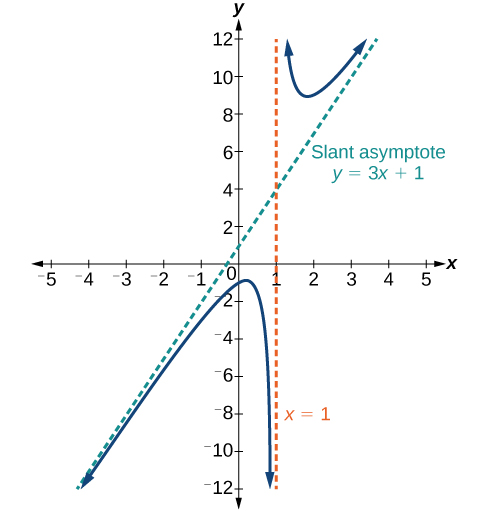
\includegraphics[scale=.9]{Chapter 5/5.6-figure1.jpeg}


\newpage
Now that we have studied all possible asymptotes (horizontal, vertical, and slanted ones), we now have all the pieces we need to graph a rational function with everything we have learned in this chapter. 

\begin{boxR}
    \textbf{Strategy for Graphing a Rational Function}
    \vspace{1mm}
    \hline
    \vspace{2mm}
    \begin{enumerate}
        \item Find the $y$ intercept (if there is one) by evaluating $f(0)$.
        \item Factor the numerator and denominator.
        \item Find the $x$-intercepts (if there are any) by solving $P(x)=0$.
        \item Find any vertical asymptotes by solving $Q(x)=0$
        \item Find the horizontal asymptote if there is one) using the rule for determining the horizontal asymptote.
        \item Find the slant asymptote if the degree of the numerator is one degree higher than the denominator.
        \item Plot at least one point in between and beyond each $x$-intercept and vertical asymptote. 
        \item Use the information to graph the function inbetween and beyond the vertical asymptotes. 
    \end{enumerate}
\end{boxR}
\vspace{5mm}

\underline{\textbf{Example 5 - Graph a Rational Function}}

\vspace{1mm}

Sketch the graph of $\D f(x)= \frac{3x^2}{x^2-4}$ by following the steps above. 

\newpage
Example 5 continued.


\newpage
\underline{\textbf{Example 6 - Graph a Rational Function}}

\vspace{1mm}

Sketch the graph of $\D f(x)= \frac{x^4}{x^2+1}$ following the steps in the strategy to graph a rational function.
\newpage

\underline{\textbf{Example 7 - Graph a Rational Function}}
\vspace{1mm}

Sketch the graph of $\D f(x)= \frac{x^2+x-30}{x-6}$ following the steps in the strategy to graph a rational function.
\newpage




\end{document}


